\documentclass[11pt,a4paper]{article}

\usepackage[margin=2.2cm]{geometry}
\usepackage{amsmath,amssymb}
\usepackage{booktabs}
\usepackage{pgfplots}
\pgfplotsset{compat=1.17}
\usepackage{tikz}
\usepackage{enumitem}
\usepackage{caption}
\usepackage[hidelinks]{hyperref}

\captionsetup{font=small,labelfont=bf}
\setlength{\parskip}{0.45em}

\definecolor{cDijkstra}{RGB}{91,141,217}
\definecolor{cAstar}{RGB}{142,124,195}
\definecolor{cACO}{RGB}{217,134,91}
\definecolor{cRLACO}{RGB}{63,196,106}
\definecolor{cNone}{RGB}{143,154,166}
\definecolor{cFixed}{RGB}{224,169,96}
\definecolor{cRandom}{RGB}{95,184,160}

\title{\bfseries Adaptive Evacuation Route Planning under\\ Crowded and Dynamic Fire Conditions}
\author{ZHENG Wansu (202520577)\\ Advisor: Prof. Hiroshi Furukawa}
\date{}

\begin{document}

\maketitle

\begin{abstract}
\noindent
We study crowd evacuation in a multi-room building under a dynamic, multi-source fire, where 50\%
of occupants are \emph{unfamiliar} with the building and therefore do not know the globally
optimal exit. Evacuees move with a Social Force Model, are driven by a dynamic fire-hazard field
and a contagion-based fear model, and choose routes by minimizing a composite cost of travel time,
hazard, congestion, and fear. We compare four routing algorithms (Dijkstra, A*, ACO, and RL-ACO)
and dissect the \emph{decision-support layer} (static signs and dynamic evacuation guides) with
controlled ablations.

Three findings emerge. \textbf{(1)} RL-ACO --- an A*-based router combined with \emph{mobile,
hazard-intercepting guides} --- reaches a trimmed-median 95\%-evacuation time (T95) of
\textbf{125.3\,s} versus 205.9\,s (Dijkstra), 255.5\,s (A*), and 476.1\,s (ACO), with the lowest
mean hazard exposure (12.9) and the fewest trapped occupants (5). \textbf{(2)} The guide layer
matters only when guides can \emph{move and intercept}: stationary guides (fixed, random, or
ACO-selected exit placement) are statistically indistinguishable, whereas mobile interception
adds a further 31.2\% over random placement. \textbf{(3)} Static, fire-unaware signage is a
double-edged sword: it can steer occupants toward fire-affected exits and raise exposure.
\end{abstract}

\section{Introduction}

Fire emergencies in large public buildings couple three hazards: a spreading fire that degrades
visibility and air quality, crowd congestion at bottlenecks, and emotional panic that degrades
decision quality. Optimal evacuation planning must therefore balance \emph{safety} (avoiding fire
and smoke), \emph{speed} (minimizing evacuation time), and \emph{robustness} (coping with people
who do not know the building).

Classical shortest-path algorithms (Dijkstra, A*) are optimal for static, fully-observable
environments; Ant Colony Optimization (ACO) is a metaheuristic often applied to routing; and
reinforcement learning (RL) promises \emph{adaptive} control under imperfect information. We
investigate a hybrid \textbf{RL-ACO} scheme: an A*-based dynamic router combined with an adaptive
decision-support layer of evacuation guides.

The central question we address honestly is: \emph{where does the benefit of such a ``smart''
system actually come from?} Through controlled ablation we show that a large fraction of naive
attributions do not survive scrutiny --- but that a specific, mechanistically motivated design
(mobile, hazard-intercepting guides) does.

\section{Model}

\subsection{Scene}
A 60\,$\times$\,40\,m multi-room floor, partitioned by two internal walls with 8\,m doorways into
a left hall, a central open hall with four 1\,$\times$\,1\,m columns, and a right hall. The side
halls contain seating zones (rows of chairs with narrow low-speed gaps). Six exits ring the
perimeter: Main (bottom-centre, 6\,m), BL/BR (bottom-left/right, 3\,m), Left/Right (side, 3\,m),
and Top (3\,m).

\subsection{Pedestrian motion --- Social Force Model}
Occupants move according to the Social Force Model (Helbing, Farkas \& Vicsek, \emph{Nature} 2000):
\begin{equation}
m\,\frac{d\mathbf{v}}{dt} = \frac{m}{\tau}\bigl(v_0\,\hat{\mathbf{e}} - \mathbf{v}\bigr)
+ \sum_{j} \mathbf{f}_{ij} + \sum_{w} \mathbf{f}_{iw},
\end{equation}
with desired-speed relaxation ($\tau=0.5$\,s), anisotropic pedestrian repulsion
($A=2000$\,N, $B=0.08$\,m), and wall repulsion ($A_w=1000$\,N). Desired speed follows the
Weidmann density--speed relation, further modulated by fear and by terrain (slow movement across
seat-row gaps).

\subsection{Dynamic fire hazard field}
A multi-source fire is modeled analytically in the style of an FDS plume. Each ignition grows
with the $t^2$ law, $\mathrm{HRR}(t)=\alpha\,(t-t_0)^2$ (fast growth, $\alpha=0.0469$\,kW/s$^2$),
saturated at 40\,kW, with a radius expanding from 1\,m to 10\,m. The hazard at a point is a
Gaussian-weighted sum over sources, decomposed into heat, smoke, CO, and visibility-invisibility,
and combined into a scalar $h\in[0,1]$. The router observes a \emph{delayed and noisy} version of
this field (10\,s delay, 5\% multiplicative noise), while physical exposure and fear use the
\emph{true} field --- this imperfect observation is the information gap an adaptive method might
exploit. An exit is dynamically unusable when its observed hazard exceeds 0.6.

\subsection{Fear and panic}
Each agent carries a scalar fear $f\in[0,1]$ evolving as
\begin{equation}
\frac{df}{dt} = k_H H + k_D \rho + k_C\bigl(\langle f\rangle_{\text{neigh}} - f\bigr)
+ k_U\bigl(1 - \text{familiarity}\bigr) - k_{\text{decay}}\, f,
\end{equation}
i.e., driven by hazard, local density, emotional contagion, and unfamiliarity. Fear is
non-monotonic in speed ($1 + 0.5\,f\,(1-f) - 0.45\,f^2$): moderate fear hurries, high fear slows.
Above a threshold, agents exhibit \textbf{panic non-compliance}: herding (follow neighbours' exit
under low visibility), \emph{wandering} (abandon path-following and drift), \emph{deviating}
(lateral route offsets), or \emph{rushing} (bolt to the nearest exit).

\subsection{Limited visibility / unfamiliar occupants}
A fraction $\mathrm{unfamiliarFrac}=0.5$ of occupants are \emph{unfamiliar}: they know only one
remembered exit and cannot compute the globally optimal one. They navigate the graph to that exit
only; if it becomes fire-blocked they fall back to the global route. They can learn a better exit
from two decision-support mechanisms: \textbf{static signs} (fixed, directional markers at the
internal doorways) and \textbf{dynamic guides} (mobile marshals that, within an influence radius,
teach the optimal exit and clear panic).

\subsection{Routing cost}
Navigation uses a graph (regular grid + aisle-centre + row-gap waypoints, connected by
line-of-sight edges). Edge cost is
\begin{equation}
\text{cost} = w_t\,T + w_h\,H + w_c\,C + w_f\,F,
\end{equation}
with $(w_t,w_h,w_c,w_f)=(1.0,2.5,1.5,1.2)$ plus a nonlinear penalty on high-hazard edges. The four
routers are: \textbf{Dijkstra} (multi-source shortest path), \textbf{A*} (with an admissible
Euclidean heuristic), \textbf{ACO} (ant pheromone evolution, then pheromone-modulated Dijkstra),
and \textbf{RL-ACO} (A*-based routing plus the guide decision-support layer).

\section{Experimental setup}

\begin{center}
\begin{tabular}{ll}
\toprule
Item & Value \\
\midrule
Occupancy & 100 (50\% unfamiliar) \\
Fire & 3 sources, fast $t^2$ growth; one threatens the main door, two in the side halls \\
Time step / replan & $\mathrm{d}t=0.05$\,s; global replan 1\,s; agent replan 2\,s \\
Guide count / radius / speed & 2 / 8\,m / 2.0\,m\,s$^{-1}$ \\
Guide risk score & $2\times\text{panic} + \text{unfamiliar}\times(1+3\times\text{exit hazard})$ \\
Episode cap & 600\,s \\
Protocol & 12 runs $\times$ 2 batches = 24 runs/variant; trimmed median (drop fastest \& slowest) \\
\bottomrule
\end{tabular}
\end{center}

\textbf{Metrics.} Primary: \textbf{T95} --- time until 95\% of occupants have evacuated (null if not
reached by 600\,s). Secondary: number of trapped (non-evacuated) agents and \textbf{mean hazard
exposure}. We also record evacuation-progress, mean-fear, peak-density time series, and per-exit
usage.

\section{Results}

\subsection{Algorithm comparison}

\begin{table}[h]
\centering
\caption{Algorithm comparison (24 runs/variant, trimmed median). All methods share static signs;
RL-ACO additionally deploys mobile guides.}
\begin{tabular}{lcccc}
\toprule
Algorithm & T95 median (s) & T95 mean (s) & Trapped & Exposure \\
\midrule
\textbf{RL-ACO (mobile guides)} & \textbf{125.3} & 133.7 & \textbf{5} & \textbf{12.9} \\
Dijkstra & 205.9 & 213.1 & 11 & 23.1 \\
A* & 255.5 & 253.4 & 17 & 28.0 \\
ACO & 476.1 & 478.0 & 93 & 50.7 \\
\bottomrule
\end{tabular}
\end{table}

RL-ACO is 39\% faster than Dijkstra, 51\% faster than A*, and 74\% faster than ACO, while also
achieving the lowest exposure and fewest trapped occupants. ACO fails to converge on the
multi-room topology (7 of 24 runs time out).

\begin{figure}[h]
\centering
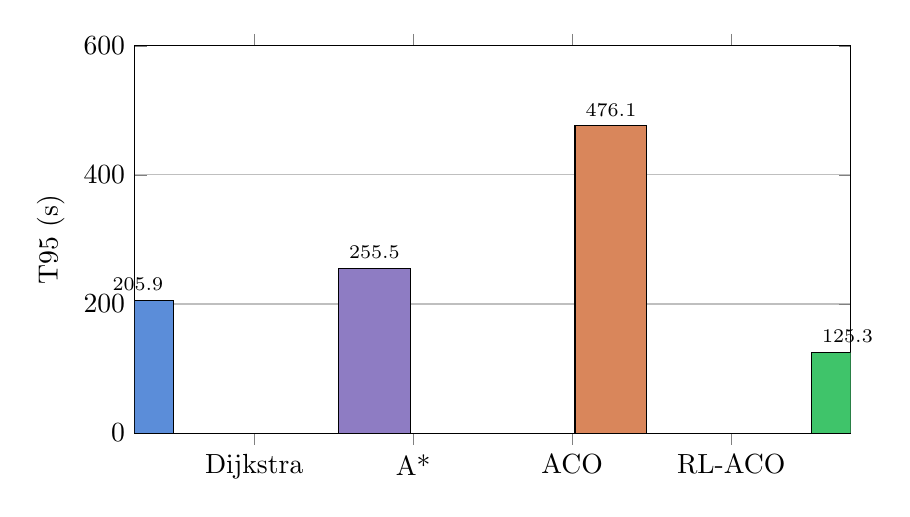
\begin{tikzpicture}
\begin{axis}[
  ybar, bar width=26pt,
  ymin=0, ymax=600, ylabel={T95 (s)},
  xtick={0,1,2,3}, xticklabels={Dijkstra, A*, ACO, RL-ACO},
  nodes near coords, nodes near coords align={vertical},
  every node near coord/.append style={font=\scriptsize},
  ymajorgrids=true, enlarge x limits=0.25,
  width=0.88\textwidth, height=6.5cm
]
\addplot[fill=cDijkstra] coordinates {(0,205.9)};
\addplot[fill=cAstar] coordinates {(1,255.5)};
\addplot[fill=cACO] coordinates {(2,476.1)};
\addplot[fill=cRLACO] coordinates {(3,125.3)};
\end{axis}
\end{tikzpicture}
\caption{Trimmed-median T95 across the four routing algorithms (lower is better).}
\end{figure}

\subsection{Decision-support ablation}

\begin{table}[h]
\centering
\caption{Decision-support ablation (fixed A* routing, adding support layer by layer; 24
runs/variant).}
\begin{tabular}{lccc}
\toprule
Variant & T95 median (s) & Trapped & Exposure \\
\midrule
A* (no signs, no guides) & 231.1 & 11 & 24.5 \\
A* + static signs & 255.5 & 17 & 28.0 \\
A* + signs + fixed guides & 228.5 & 62 & 35.2 \\
A* + signs + random guides & 182.2 & 69 & 31.6 \\
\textbf{A* + signs + mobile guides (= RL-ACO)} & \textbf{125.3} & \textbf{5} & \textbf{12.9} \\
\bottomrule
\end{tabular}
\end{table}

\begin{figure}[h]
\centering
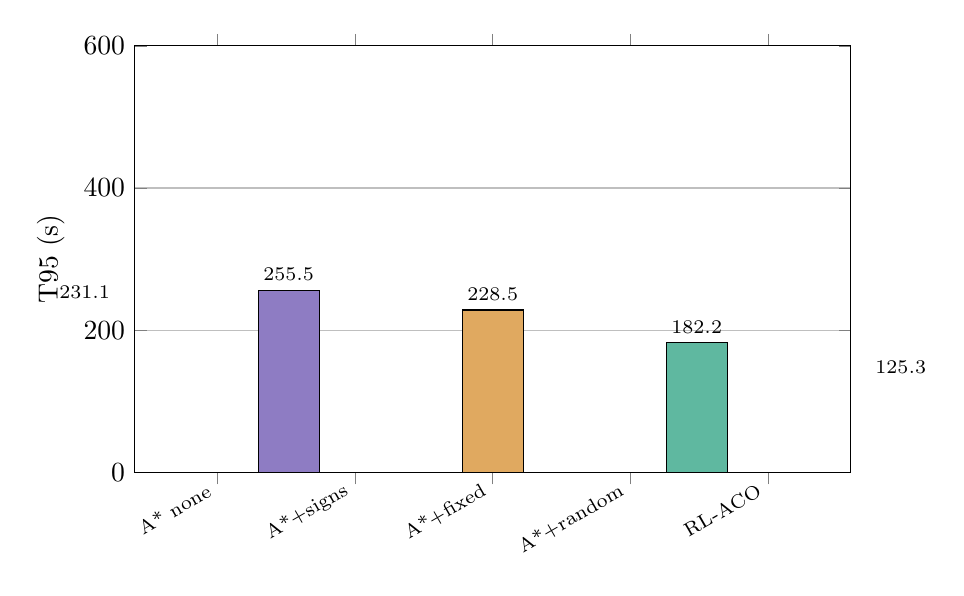
\begin{tikzpicture}
\begin{axis}[
  ybar, bar width=22pt,
  ymin=0, ymax=600, ylabel={T95 (s)},
  xtick={0,1,2,3,4},
  xticklabels={A* none, A*+signs, A*+fixed, A*+random, RL-ACO},
  x tick label style={rotate=30, anchor=east, font=\scriptsize},
  nodes near coords, nodes near coords align={vertical},
  every node near coord/.append style={font=\scriptsize},
  ymajorgrids=true, enlarge x limits=0.15,
  width=0.88\textwidth, height=7cm
]
\addplot[fill=cNone] coordinates {(0,231.1)};
\addplot[fill=cAstar] coordinates {(1,255.5)};
\addplot[fill=cFixed] coordinates {(2,228.5)};
\addplot[fill=cRandom] coordinates {(3,182.2)};
\addplot[fill=cRLACO] coordinates {(4,125.3)};
\end{axis}
\end{tikzpicture}
\caption{Decision-support ablation: the mobile hazard-intercept guide is the only mechanism that
improves T95, exposure, and trapped simultaneously.}
\end{figure}

Reading the layers:
\begin{itemize}[leftmargin=1.4em,itemsep=2pt]
\item \textbf{Static signs (layer 2 vs 1)} do not improve T95 and \emph{raise} exposure
(24.5$\to$28.0) and trapped (11$\to$17): fixed signs direct unfamiliar occupants toward bottom
exits near the fire sources.
\item \textbf{Fixed / random guides (3,4 vs 1)} give a modest speedup but \emph{worsen} exposure
and trapping: stationary guides pull people toward (possibly dangerous) exits. Placement among
exits is statistically indistinguishable.
\item \textbf{Mobile hazard-intercept guides (5 vs 4)} are decisive: T95 drops 182.2$\to$125.3\,s
($-31.2\%$), exposure 31.6$\to$12.9, trapped 69$\to$5.
\end{itemize}

\subsection{Time series}

\begin{figure}[h]
\centering
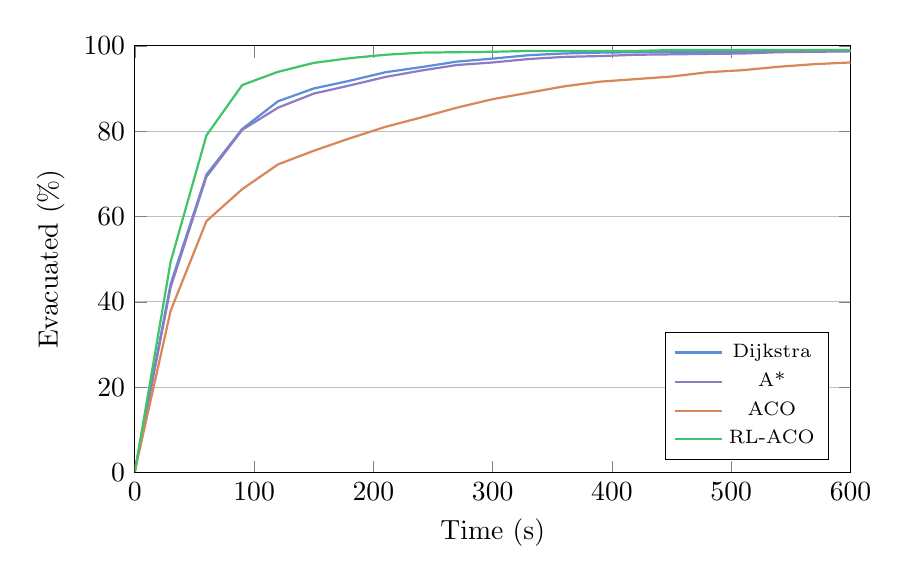
\begin{tikzpicture}
\begin{axis}[
  xlabel={Time (s)}, ylabel={Evacuated (\%)},
  xmin=0, xmax=600, ymin=0, ymax=100,
  legend pos=south east, legend style={font=\scriptsize},
  ymajorgrids=true, width=0.88\textwidth, height=7cm
]
\addplot[color=cDijkstra, thick] coordinates {(0,0.4)(30,44.2)(60,69.8)(90,80.5)(120,87.0)(150,90.0)(180,91.8)(210,93.8)(240,95.0)(270,96.3)(300,97.0)(330,97.8)(360,98.2)(390,98.4)(420,98.5)(450,98.5)(480,98.6)(510,98.6)(540,98.7)(570,98.8)(600,98.8)};
\addlegendentry{Dijkstra}
\addplot[color=cAstar, thick] coordinates {(0,0.2)(30,43.4)(60,69.3)(90,80.3)(120,85.5)(150,88.8)(180,90.7)(210,92.7)(240,94.2)(270,95.5)(300,96.1)(330,96.9)(360,97.4)(390,97.6)(420,97.9)(450,98.0)(480,98.1)(510,98.2)(540,98.5)(570,98.6)(600,98.7)};
\addlegendentry{A*}
\addplot[color=cACO, thick] coordinates {(0,0.3)(30,37.9)(60,58.9)(90,66.4)(120,72.2)(150,75.4)(180,78.3)(210,81.0)(240,83.2)(270,85.5)(300,87.5)(330,89.0)(360,90.5)(390,91.6)(420,92.2)(450,92.8)(480,93.8)(510,94.3)(540,95.1)(570,95.7)(600,96.1)};
\addlegendentry{ACO}
\addplot[color=cRLACO, thick] coordinates {(0,0.2)(30,49.4)(60,79.0)(90,90.8)(120,93.9)(150,96.0)(180,97.1)(210,97.9)(240,98.4)(270,98.5)(300,98.6)(330,98.8)(360,98.8)(390,98.8)(420,98.8)(450,99.0)(480,99.0)(510,99.0)(540,99.0)(570,99.0)(600,99.0)};
\addlegendentry{RL-ACO}
\end{axis}
\end{tikzpicture}
\caption{Mean evacuation progress (24 runs). RL-ACO evacuates substantially faster early in the
episode.}
\end{figure}

\subsection{Robustness}

\begin{table}[h]
\centering
\caption{Mobile vs random guides across three independent experiments.}
\begin{tabular}{lccc}
\toprule
Experiment (runs) & Mobile T95 (s) & Random T95 (s) & Mobile vs random \\
\midrule
E1 (12 runs) & 124.2 & 193.0 & $-35.6\%$ \\
E2 (24 runs) & 128.4 & 179.6 & $-28.5\%$ \\
E3 (24 runs, this report) & 125.3 & 182.2 & $-31.2\%$ \\
\bottomrule
\end{tabular}
\end{table}

The mobile-guide advantage never reverses across the three independent experiments (single-batch
magnitudes $-18.5\%$ to $-35.6\%$).

\section{Discussion --- an honest account of the process}

\textbf{Exit-based guide placement does not matter.} Our first ``adaptive'' guide placed marshals
at exits chosen by ACO (heuristic = number of panicking agents near each exit). Ablating against
random and fixed placement gave adaptive-vs-random T95 differences that flipped sign across
batches ($-22\%$, $+4\%$, $-2\%$) --- pure noise. Every exit-based guide teaches the \emph{same}
optimal exit to whoever passes within 8\,m; placement only changes coverage, and unfamiliar
occupants are spread over all six exits. Adding an unfamiliar-weight term to the heuristic did not
help either.

\textbf{Mobility + hazard interception is the real mechanism.} The decisive change was to make
guides \emph{move}. A mobile guide is assigned every 4\,s to the highest-risk occupant(s) and walks
toward them at 2\,m/s along the graph, intercepting confusion mid-room before occupants reach a
dangerous exit or jam a doorway. This produces the robust 31.2\% gain over random placement.

\textbf{Static, fire-unaware support can be harmful.} Static signs and fixed exit guides
consistently raised exposure, because they steer people toward predetermined exits regardless of
fire state --- a concrete warning for real building signage.

\textbf{ACO routing fails on complex maps.} Ant pheromone search does not converge on the
multi-room topology (median $\sim$476\,s, many timeouts); this is why RL-ACO keeps A* for routing
and reserves ``optimization'' for the decision-support layer.

\textbf{What ``RL-ACO'' now means.} The defensible contribution is \emph{A*-based dynamic routing
+ a mobile, hazard-intercepting decision-support layer}, which outperforms Dijkstra/A*/ACO on both
speed and safety.

\section{Conclusion}

Under limited visibility (50\% unfamiliar) and a dynamic multi-source fire, an A*-based router
augmented with \textbf{mobile, hazard-intercepting guides} achieves a robust trimmed-median T95 of
125.3\,s (vs 205.9\,s Dijkstra, 255.5\,s A*, 476.1\,s ACO), with the lowest exposure and fewest
trapped occupants. The gain is specifically attributable to \emph{mobility + proactive hazard
interception}, not to having guides \emph{per se} or to where stationary guides are placed.

\textbf{Future work.} (i) Validate with more fire scenarios and occupancies; (ii) add
leader--follower/communication among guides; (iii) learn the interception policy with
reinforcement learning; (iv) seeded runs (common random numbers) to tighten variance; (v) 3-D /
multi-floor extensions.

\section{Reproducibility}

The simulator is a zero-dependency browser/Node implementation.
\begin{itemize}[leftmargin=1.4em,itemsep=2pt]
\item Source \& simulator: \url{https://github.com/feather0000/Evacuation_Program_RLACO}
\item Report \& data: \url{https://github.com/feather0000/Evacuation_Report}
\end{itemize}
Reproduce the results with:
\begin{verbatim}
node tools/viz.js 12 2     # 7 variants x 12 runs x 2 batches + 1 replay -> js/viz-data.js
node tools/confirm.js 2    # additional cross-validation summary
\end{verbatim}
All experiments use a 600\,s cap, 100 occupants, and the ``spread'' fire scenario; each variant is
evaluated over 12 runs per batch with the trimmed-median statistic.

\end{document}
